\documentclass[a4paper,12pt]{article}
\usepackage{amsmath, amsthm, amssymb}
\usepackage{tikz} % 添加绘图
\usepackage{tabularx}
\usepackage{enumitem}
\usepackage{fancyref}

\usepackage[top=1in,bottom=1in,left=1in,right=1in]{geometry} % 用于设置页面布局
\usepackage{xeCJK} % 用于使用本地字体
\usepackage[super, square, sort&compress]{natbib} % 处理参考文献
\usepackage{titlesec, titletoc} % 设置章节标题及页眉页脚
%\usepackage{xCJKnumb} % 中英文数字转换
\usepackage{amssymb}
\usepackage{amsmath} % 在公式中用\text{文本}输入中文
\usepackage{diagbox}
\usepackage{multirow} % 表格中使用多行
\usepackage{booktabs} % 表格中使用\toprule等命令
\usepackage{rotating} % 使用sidewaystable环境旋转表格
\usepackage{tabularx}
\usepackage{graphicx} % 处理图片
\usepackage{footnote} % 增强的脚注功能,可添加表格脚注
\usepackage{threeparttable} % 添加真正的表格脚注,示例见README
\usepackage{hyperref} % 添加pdf书签

\usepackage{tikz}
\usetikzlibrary{shapes,arrows,shadows}

% 字体设置
\setmainfont{Times New Roman}
\setsansfont[Scale=MatchLowercase,Mapping=tex-text]{PT Sans}
\setmonofont[Scale=MatchLowercase]{PT Mono}
\setCJKmainfont[ItalicFont={Kaiti SC}, BoldFont={Heiti SC}]{Songti SC}
\setCJKsansfont{Heiti SC}
\setCJKmonofont{Songti SC}
% \setCJKmainfont[BoldFont={FZXiaoBiaoSong-B05S}]{Songti SC}
% \setCJKfamilyfont{kai}[BoldFont=Heiti SC]{Kaiti SC}
% \setCJKfamilyfont{song}[BoldFont=Heiti SC]{Songti SC}
% \setCJKfamilyfont{hei}[BoldFont=Heiti SC]{Heiti SC}
% \setCJKfamilyfont{fsong}[BoldFont=Heiti SC]{Songti SC}
% \newcommand{\kai}[1]{{\CJKfamily{kai}#1}}
% \newcommand{\hei}[1]{{\CJKfamily{hei}#1}}
% \setromanfont[Mapping=tex-text]{TeXGyrePagella}
% \setsansfont[Scale=MatchLowercase,Mapping=tex-text]{TeXGyrePagella}
% \setmonofont[Scale=MatchLowercase]{Courier New}
%%设置常用中文字号,方便调用
\newcommand{\erhao}{\fontsize{22pt}{\baselineskip}\selectfont}
\newcommand{\xiaoerhao}{\fontsize{18pt}{\baselineskip}\selectfont}
\newcommand{\sanhao}{\fontsize{16pt}{\baselineskip}\selectfont}
\newcommand{\xiaosanhao}{\fontsize{15pt}{\baselineskip}\selectfont}
\newcommand{\sihao}{\fontsize{14pt}{\baselineskip}\selectfont}
\newcommand{\xiaosihao}{\fontsize{12pt}{\baselineskip}\selectfont}
\newcommand{\wuhao}{\fontsize{10.5pt}{\baselineskip}\selectfont}
\newcommand{\xiaowuhao}{\fontsize{9pt}{\baselineskip}\selectfont}
\newcommand{\liuhao}{\fontsize{7.5pt}{\baselineskip}\selectfont}

% 章节标题显示方式及页眉页脚设置
% \item xCJKnumb是自己额外安装的包
% \item titleformat命令定义标题的形式
% \item titlespacing定义标题距左、上、下的距离
\titleformat{\section}{\raggedright\large\bfseries}{\thesection}{1em}{}
\titleformat{\subsection}{\raggedright\normalsize\bfseries}{\thesubsection}{1em}{}
\titlespacing{\section}{0pt}{*0}{*2}
\titlespacing{\subsection}{0pt}{*0}{*1}
% 由于默认的2em缩进不够,所以我手动调整了,但是在windows下似乎2.2就差不多了,或者是article中没有这个问题
\setlength{\parindent}{2.2em}

% 设置表格标题前后间距
\setlength{\abovecaptionskip}{0pt}
\setlength{\belowcaptionskip}{0pt}


\renewcommand{\refname}{\bfseries{参~考~文~献}} %将Reference改为参考文献(用于 article)
% \renewcommand{\bibname}{参~考~文~献} %将bibiography改为参考文献(用于 book)
\renewcommand{\baselinestretch}{1.38} %设置行间距
\renewcommand{\figurename}{\small\ttfamily 图}
\renewcommand{\tablename}{\small\ttfamily 表}

\setlength{\parindent}{0em}

\newtheorem{definition}{定义}
\newtheorem{lemma}{引理}
\newtheorem{proposition}{命题}
\newtheorem{program}{程序}
\newtheorem{convention}{约定}
\renewcommand*{\proofname}{证明}

\title{关于理解伴随的几种思路}
\author{苑明理}
\date{2018年12月}

\begin{document}

\maketitle{}

\renewcommand\contentsname{目录}
\setcounter{tocdepth}{2}
\tableofcontents

\newpage

\section{问题的提出}

伴随出现在许多数学领域,它在最优控制、敏感分析、变分同化中都扮演了重要的角色。近来在深度学习同微分方程结合的方向上,人们也发现了伴随的重要价值。
在学习、理解伴随概念的过程中,我们整理出在相关领域文献里三种推导伴随的思路,并认为这些思路应该是统一的。

\subsection{基本定义及几何解释}

\begin{definition}
\label{d0}
两个向量空间 $X$、$Y$ 通过一个到域 $ F $ 的双线性映射 $ \langle , \rangle : X \times Y \to F $ 构成一个对偶系统 $ \langle X, Y \rangle $。
\end{definition}

对偶系统的一个例子是 $ E^3 $ 和其上的一个标架系统 $ (x, y, z) $ 。借鉴这个例子,我们做如下约定:

\begin{convention}
称呼对偶系统 $ \langle X, Y \rangle $ 中的 $ X $ 为底空间, $ Y $ 为标架空间,$ \langle x, y \rangle $ 的值为坐标。
\end{convention}

在日常生活中,我们都有如下的经验

\begin{figure}[ht]
\centering
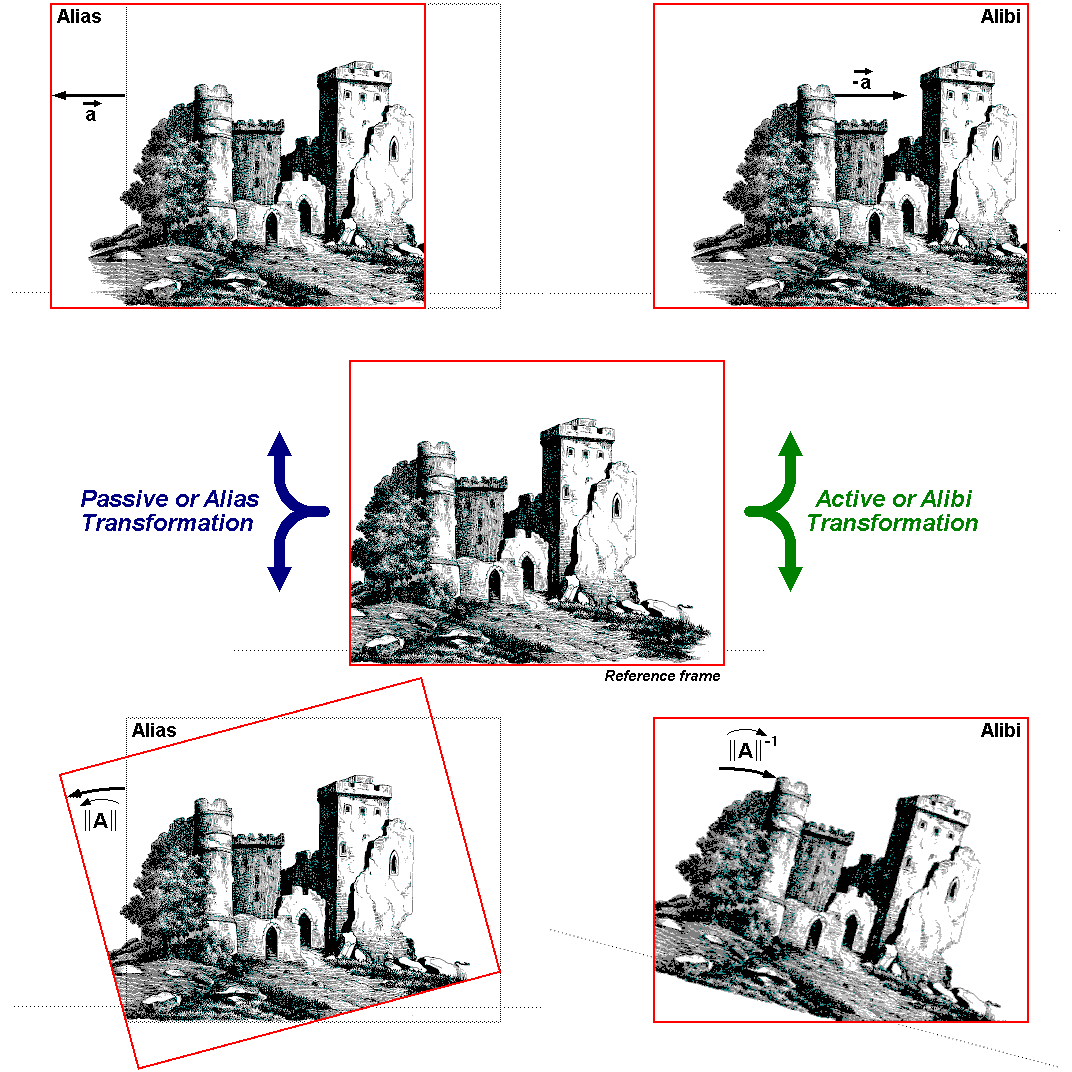
\includegraphics[width=3.5in]{images/adjoint/alias_and_alibi.png}
\caption{互为伴随的两个映射}
\end{figure}

仔细体会上述体验的内涵,我们就到达了伴随这一概念。

\begin{definition}
\label{d1}
考虑两个对偶系统 $ \langle X_1, Y_1 \rangle $ 和 $ \langle X_2, Y_2 \rangle $ ,两个算符 $ A : X_1 \to X_2$ 和  $B : Y_2 \to Y_1 $ 称为互为伴随的,
当且仅当,对任意的 $ \phi \in X_1 $ 和 $ \psi \in Y_2 $ 下式得到满足:$$ \langle A \phi, \psi \rangle = \langle \phi, B \psi \rangle $$
\end{definition}

\subsection{一般的约束优化问题}

\subsection{一类含时的约束优化问题}

\section{第一种推导思路}

\section{第二种推导思路}

\section{第三种推导思路}

\section{进一步讨论}

\subsection{三种思路的关系}

\subsection{伴随方法的优点}

\end{document}
